% Editorial preview. All new empirical outcomes below are hypothetical.
% Build: latexmk -xelatex -outdir=/tmp/serve-preview preview.tex
\documentclass{article}
\usepackage{vendor/iclr2027/iclr2027_conference}
\usepackage{fontspec}
\setmainfont{Times New Roman}
\setsansfont{Times New Roman}
\setmonofont{Times New Roman}
\font\iclrtenhv="Times New Roman/B" at 8pt
\usepackage[protrusion=true,expansion=false]{microtype}
\usepackage{amsmath,amssymb,amsthm,booktabs,array,graphicx,xcolor,placeins,xurl}
% The ICLR template requests one line of space after each table title.
\AddToHook{env/table/begin}{\setlength{\belowcaptionskip}{11pt}\setlength{\tabcolsep}{3pt}}
\usepackage[hidelinks,hypertexnames=false]{hyperref}
\hypersetup{pdftitle={SERVE: hypothetical completed-study editorial preview},
 pdfsubject={All new empirical results are illustrative, not measured research findings.}}
\urlstyle{same}
\newcommand{\R}{\mathbb{R}}
\newcommand{\E}{\mathbb{E}}
\newcommand{\ind}{\mathbf{1}}
\newtheorem{proposition}{Proposition}
\title{SERVE: Semantic Evidence from Return\\Verification for LiDAR Segmentation}
\author{Anonymous authors}
\lhead{Under review as a conference paper at ICLR 2027}
\begin{document}
\maketitle

\begin{abstract}
An unfamiliar object can receive a confident semantic label when a LiDAR model only compares known classes. We propose Semantic Evidence from Return Verification (SERVE), a model that asks whether a candidate class also predicts the observed range from its surroundings. A full-scan encoder supplies appearance support, while a separate predictor excludes the target angular cell and produces a class-conditioned distribution over log range. The likelihood of the held-out measurement enters the supervised class decision alongside appearance support. The strongest joint class support supplies both the semantic label and the unknown score. Training uses normal semantic labels and recorded ranges. On STU, SERVE reaches 78.64\% validation and 67.21\% test average precision, compared with 21.36\% and 15.09\% for a matched appearance model, while improving normal semantic mIoU by 2.15 points. At a 1\% normal false-positive rate, it recovers 88.4\% of unknown points confidently assigned to known classes by the appearance model. Matched ablations isolate the contributions of target exclusion, class-conditioned measurement support, and joint semantic training. These results support using predicted physical observations as evidence within semantic recognition.
\end{abstract}

\section{Introduction}
LiDAR segmentation must recognize familiar traffic participants while identifying objects outside its training vocabulary. A classifier can confidently label an unfamiliar road obstacle as a car or road because confidence expresses a preference among the available classes. Assessing how well a candidate class explains the observation provides additional evidence for detecting such obstacles. Real road-anomaly benchmarks such as STU make this distinction consequential for dense perception \citep{stu}.

Existing methods estimate unknownness from classifier outputs, normal feature structure, or auxiliary anomalous examples \citep{energy,pixood,lido,ndp}. An additional source of evidence is available in a LiDAR scan: the observed range is constrained by the surfaces around it. Under a road hypothesis, surrounding ground returns constrain where a held-out ray should intersect the surface. A nearer measurement weakens that hypothesis. However, a normal car can also produce a nearer return. Geometry becomes useful for recognition when each candidate class is allowed its own explanation, and the same class must support both the observed appearance and the measured range.

We introduce Semantic Evidence from Return Verification (SERVE). For every point, a full-scan encoder supplies appearance support for each known class. A separate context encoder predicts a range distribution for each class from neighboring angular cells. Evaluating these predictions at the held-out target range produces measurement support. SERVE combines the two supports within each class and uses the resulting energies for both semantic labeling and unknown detection. Normal semantic labels supervise this combined decision, training the range predictor through semantic competition.

The prediction target is a recorded physical measurement that stays fixed while the semantic representation learns. The predictor excludes the complete target cell before any cross-cell interaction, so its prediction depends on surrounding returns and the candidate class. A normalized predictive distribution accounts for both residual error and predictive spread: broad predictions accommodate variation at the cost of lower peak density. Normal likelihood and appearance compactness objectives train absolute support, complementing the relative class preferences learned by cross-entropy.

SERVE brings class-conditioned prediction of held-out physical measurements into dense semantic recognition. Its decision rule retains disagreement between appearance and measurement evidence whenever the two favor different classes. We derive this relationship and evaluate the model through matched training and fixed-weight inference comparisons. Under matched normal training data, SERVE improves STU test AP by 52.12 points over its appearance control. Removing measurement evidence from class supervision reduces validation AP by 30.37 points, showing that predictive fitting and joint semantic learning play complementary roles.

\section{Related Work}
\paragraph{Open-world LiDAR perception.}
Classifier confidence and energy provide inexpensive unknown scores \citep{msp,energy}. RbA and PixOOD develop class rejection and normal-feature modeling for dense perception \citep{rba,pixood}; LIDO uses prototype geometry for normal-only LiDAR anomaly segmentation \citep{lido}. Other methods train with auxiliary anomalous observations: REAL scales objects, LiON introduces diverse synthetic objects, DOODLE generates examples with diffusion, and NDP combines synthetic geometry with a learned prior over network predictions \citep{real,lion,doodle,ndp}. COVAL varies the visibility of generated anomalies to learn consistent representations \citep{coval}. SERVE learns from normal semantic labels and recorded ranges, using neighboring returns to test each class's prediction of a held-out measurement. Target exclusion defines the information available to this predictor.

\paragraph{Reconstruction as class support.}
C2AE conditions reconstruction on class hypotheses, and CoReSeg extends class-conditioned reconstruction to open-set segmentation \citep{c2ae,coreseg}. CSSR uses class-specific autoencoders to reconstruct learned semantic features and trains classification through reconstruction-error logits \citep{cssr}. SERVE uses a fixed physical target: it predicts the recorded range from target-excluded context and combines the resulting normalized conditional density with appearance support. This choice ties class evidence to an observable quantity throughout representation learning. Joint energy models share class scores between recognition and generative learning over complete inputs \citep{jem}. SERVE combines an appearance support function and a conditional measurement density in a discriminative class energy.

\paragraph{Prediction from restricted context.}
Blind-spot self-supervision excludes an observation before predicting it \citep{noise2self,blindspot,pn2v}. Conditional neural processes parameterize distributions at queries from observed context \citep{cnp,anp}, and masked point-cloud learning exploits spatial prediction objectives \citep{pointmae}. SERVE applies restricted-context prediction to semantic recognition: each class predicts the target return, and its density at the recorded range contributes to the class decision. Proper scoring rules provide the basis for normal likelihood fitting \citep{proper}. Studies of generative likelihood show that anomaly rankings depend on the modeled observation and its coordinates \citep{likelihood,perfectdensity}; SERVE specifies log range as its target and evaluates measurement support jointly with appearance.

\section{Semantic Evidence from Return Verification}
\label{sec:method}
\subsection{One Support Function for Labeling and Rejection}
A scan is $X=\{(\mathbf x_i,I_i)\}_{i=1}^{N}$, with position $\mathbf x_i$ and intensity $I_i$. Write $r_i=\|\mathbf x_i\|_2$, $\boldsymbol\omega_i=\mathbf x_i/r_i$, and $z_i=\log(r_i/r_0)$ with $r_0=1$\,m. The known vocabulary is $\mathcal C=\{1,\ldots,C\}$. A normal training label specifies either a class or an allowed set $Y_i\subseteq\mathcal C$ when source labels are coarser than the target vocabulary.

For each class $c$, SERVE computes appearance support $a_{ic}\in(0,1]$ and a log-range density $p_{ic}=p_\theta(z_i\mid C_i,\boldsymbol\omega_i,c)$ from target-excluded context $C_i$. Let $M$ bound the density and $\kappa_i$ indicate whether any prescribed context cell is available. Define
\begin{equation}
 s_{ic}=-\log a_{ic},\qquad
 g_{ic}=\kappa_i(\log M-\log p_{ic}),\qquad
 E_{ic}=s_{ic}+g_{ic}.
 \label{eq:energy}
\end{equation}
The class support is $v_{ic}=\exp(-E_{ic})$. The semantic prediction and unknown score are
\begin{equation}
 \hat y_i=\arg\min_c E_{ic},\qquad u_i=\min_c E_{ic}.
 \label{eq:decision}
\end{equation}
A point is rejected when $u_i$ exceeds a threshold. With no neighboring cell, $g_{ic}=0$ for all classes and inference uses appearance support alone.

\begin{figure}[t]
\centering
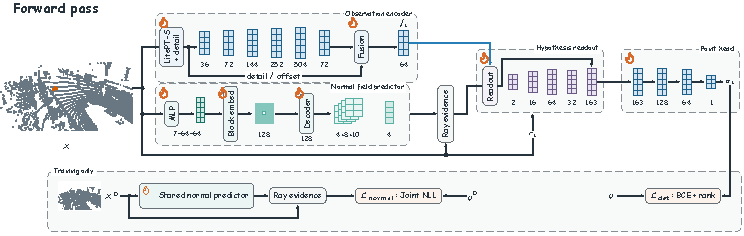
\includegraphics[width=\linewidth]{figures/method.pdf}
\caption{SERVE. The full-scan branch produces appearance support. Independently encoded neighboring cells supply a separate predictor. Each class predicts a distribution over the held-out target's log range. Combining its density at the measured range with appearance support yields the semantic label, unknown score, and supervised class probabilities. The indicator $\kappa_i$ selects appearance-only inference for empty context. A recorded input scan and schematic density curves illustrate the computation.}
\label{fig:method}
\end{figure}

\paragraph{Same-class evidence combination.}
Let $s_i^*=\min_c s_{ic}$ and $g_i^*=\min_c g_{ic}$. Then
\begin{equation}
 u_i=s_i^*+g_i^*+\Delta_i,\qquad
 \Delta_i=\min_c[(s_{ic}-s_i^*)+(g_{ic}-g_i^*)]\geq0.
 \label{eq:gap}
\end{equation}
The additional term vanishes exactly when at least one class minimizes both energies. Independently taking the best appearance and the best measurement explanation drops $\Delta_i$, even when they belong to different classes. For example, appearance supports $(0.9,0.1)$ and measurement supports $(0.1,0.9)$ produce a best same-class product of $0.09$, versus $0.81$ after independent maximization. Same-class combination therefore increases the unknown score when appearance and measurement favor incompatible explanations.

\subsection{Appearance and Conditional Return Prediction}
\paragraph{Multimodal appearance.}
A LitePT-S backbone \citep{litept} encodes the scan with $5$\,cm voxels. Point features derived from coordinates, intensity, and within-voxel offsets preserve detail lost by voxel aggregation. Concatenating both representations gives an embedding $\mathbf h_i\in\R^D$, $D=48$. A shared class vector $\mathbf q_c$ and $A=4$ offsets represent normal variation:
\begin{equation}
 \mathbf t_{cm}=\sqrt D\frac{\mathbf q_c+\boldsymbol\delta_{cm}}{\|\mathbf q_c+\boldsymbol\delta_{cm}\|_2},\qquad
 a_{ic}=\frac1A\sum_{m=1}^{A}\exp\!\left(-\frac{\|\mathbf h_i-\mathbf t_{cm}\|_2^2}{D\tau}\right),
 \label{eq:appearance}
\end{equation}
with $\tau=0.2$. Common norms, temperature, and mode count set a shared scale. The same class vectors query the measurement predictor and receive gradients from both branches under the joint objective.

\paragraph{Excluding the target before prediction.}
Azimuth and elevation partition returns into $0.5^\circ$ cells. A separate pointwise encoder processes raw returns, and independent within-cell mean/max pooling produces one token per occupied cell. For a target cell, two cross-attention layers query eight neighboring offsets at each of radii one and three cells, giving 16 context positions. Queries contain the candidate class and target angular position. The predictor receives only these neighboring tokens and queries; all target-cell returns are excluded before cross-cell interaction. After predicting the distribution parameters, the model evaluates the density at the target's recorded range. This order holds for every return in the target cell, including multiple returns along nearby directions.

\paragraph{Predicting a distribution of log ranges.}
Each class predicts a $K=3$ component Student-$t$ mixture with three degrees of freedom. For target cell $j$, ray offsets $(d_a,d_e)$ normalized by the half-cell width define $\boldsymbol\phi_i=(d_a,d_e,d_a^2,d_ad_e,d_e^2)$. The component means and scales are
\begin{equation}
 \mu_{ick}=\bar z_{C_j}+\alpha_{jck}+\boldsymbol\beta_{jck}^{\mathsf T}\boldsymbol\phi_i,
 \qquad \sigma_{jck}=\sigma_{\min}+\operatorname{softplus}(\rho_{jck}),
 \label{eq:surface}
\end{equation}
where $\bar z_{C_j}$ averages neighboring cells' mean log ranges and $\sigma_{\min}=10^{-3}$. Softmax weights $w_{jck}$ define
\begin{equation}
 p_{ic}=\sum_{k=1}^{K}w_{jck}\frac{2}{\pi\sqrt3\,\sigma_{jck}}
 \left(1+\frac{(z_i-\mu_{ick})^2}{3\sigma_{jck}^2}\right)^{-2}.
 \label{eq:density}
\end{equation}
Each mixture integrates to one in log-range space and is bounded by $M=2/(\pi\sqrt3\,\sigma_{\min})$. Hence all energies in Equation~\eqref{eq:energy} are nonnegative. Increasing a component's scale tenfold reduces its peak density tenfold, so measurement support accounts for predictive spread as well as residual error. Multiple components represent alternative surface continuations.

\subsection{Training Measurement Evidence through Semantic Competition}
Semantic supervision uses $P_{ic}=\operatorname{softmax}_c(-E_{ic})$ and an allowed-set loss:
\begin{equation}
 \ell_{\mathrm{joint},i}=-\log\sum_{c\in Y_i}P_{ic},\qquad
 \frac{\partial\ell_{\mathrm{joint},i}}{\partial\log p_{ic}}
 =\kappa_i(P_{ic}-P^Y_{ic}),
 \label{eq:joint}
\end{equation}
where $P^Y_{ic}=\ind[c\in Y_i]P_{ic}/\sum_{d\in Y_i}P_{id}$ and the partial derivative holds the other intermediate inputs fixed. For a fine label, the true class receives a likelihood-increasing gradient and competing classes receive the opposite gradient. Measurement prediction thereby participates directly in the semantic decision.

Cross-entropy depends on relative energies: adding the same scalar to every class leaves $P_{ic}$ unchanged but shifts $u_i$. We therefore also train absolute support. Context logits $\eta_{ic}$ define weights $\pi^Y_{ic}=\exp\eta_{ic}/\sum_{d\in Y_i}\exp\eta_{id}$ over allowed classes. The predictive and compactness losses are
\begin{equation}
 \ell_{\mathrm{pred},i}=-\log\sum_{c\in Y_i}\pi^Y_{ic}p_{ic},\qquad
 \ell_{\mathrm{compact},i}=-\log\left(\frac1{|Y_i|}\sum_{c\in Y_i}a_{ic}\right).
 \label{eq:absolute}
\end{equation}
For fine labels, predictive training is true-class negative log likelihood (NLL). For coarse labels, it fits the mixture over the allowed classes. An appearance classification loss uses $\operatorname{softmax}(-s)$, and a context classification loss uses $\operatorname{softmax}(\eta)$, both with the same allowed-set formulation. The full objective is
\begin{equation}
 \mathcal L=\mathcal L_{\mathrm{joint}}+0.5\mathcal L_{\mathrm{appearance}}
 +0.05\mathcal L_{\mathrm{compact}}+0.2\mathcal L_{\mathrm{pred}}
 +0.2\mathcal L_{\mathrm{context}}.
 \label{eq:loss}
\end{equation}
Classification losses balance distinct allowed label sets within each frame. Joint supervision uses up to $4{,}096$ normal queries; the appearance loss covers all reliably labeled points. Predictive and context losses exclude queries with $\kappa_i=0$. Appendix~\ref{app:training} gives exact reductions.

The objective trains normalized conditional densities for a discriminative decision: predictive NLL rewards fit to normal ranges, while semantic cross-entropy rewards class separation. Their combined effect determines the fitted distribution. Appendix~\ref{app:theory} derives this interaction, and Section~\ref{sec:experiments} evaluates the resulting predictive coverage and anomaly ranking. The combined quantity $v_{ic}$ represents class support.

\section{Experiments}
\label{sec:experiments}
\subsection{Evaluation Design}
\paragraph{Normal training and selection.}
We use $28{,}130$ nuScenes training scans from $700$ scenes, with scene-disjoint normal development data \citep{nuscenes}, and $449$ normal STU scans from sequence 206. The output vocabulary contains 19 normal STU classes. Source labels map to compatible target-class sets; supplementary source annotations refine selected rider, parking, and building labels. All matched models receive identical supervision. Training uses two source passes followed by eight target passes with one source replay scan per four target scans. LitePT-S starts from official nuScenes-pretrained weights. Model selection uses normal semantic mIoU, with the normal objective breaking ties. Anomaly labels are reserved for evaluation. Appendix~\ref{app:training} specifies annotations, optimization, and three paired random seeds.

\paragraph{Metrics and populations.}
We report normal development mIoU over the 14 classes present in STU sequence 201, and anomaly AP, AUROC, and FPR95 on STU validation and hidden test. Official point evaluation retains distances from $2.5$ to $50$\,m, applies the benchmark label mask, and includes a scan when it contains at least five valid anomaly points \citep{stu}. Objects with one to four points remain included in eligible scans. Metrics pool valid point predictions before reduction. Fixed-FPR comparisons set each model's threshold on the same evaluation normal population, giving a shared false-alarm budget.

\paragraph{Matched controls.}
The appearance control is independently trained using appearance classification and compactness. The separate-objectives control retains SERVE's architecture, shared class vectors, predictive losses, and joint inference, and uses appearance support alone in the classification loss. This comparison tests direct supervision of measurement evidence through class competition. Our dense adaptation of CSSR reconstructs backbone features with class-specific autoencoders and uses reconstruction errors as class logits. Standard softmax and energy use a linear class head. Matched runs share backbone initialization, scan order, normal supervision, and update budget. Full definitions appear in Appendix~\ref{app:controls}.

\subsection{Unknown Detection and Normal Perception}
\begin{table}[t]
\caption{Normal development mIoU and point-level anomaly detection (\%). The upper block reports three-seed means under matched normal-only training; bold marks its best results. The lower block reports published results with each method's original backbone, training data, and supervision: LIDO \citep{lido}, NDP \citep{ndp}, and COVAL \citep{coval}. COVAL's ML and AL scores occupy separate rows; n/r denotes an unreported value.}
\label{tab:main}
\centering
\begin{tabular}{lrrrrrrr}
\toprule
 & 201 & \multicolumn{3}{c}{STU validation} & \multicolumn{3}{c}{STU test}\\
\cmidrule(lr){3-5}\cmidrule(lr){6-8}
Model & mIoU$\uparrow$ & AP$\uparrow$ & AUROC$\uparrow$ & FPR95$\downarrow$ & AP$\uparrow$ & AUROC$\uparrow$ & FPR95$\downarrow$\\
\midrule
\multicolumn{8}{l}{Matched normal-only training}\\
Softmax & 61.84 & 12.60 & 96.40 & 20.84 & 7.31 & 95.05 & 25.47\\
Energy & 61.84 & 18.72 & 97.12 & 16.35 & 12.64 & 96.51 & 20.08\\
Appearance & 61.92 & 21.36 & 97.86 & 12.48 & 15.09 & 97.05 & 16.22\\
CSSR-style & 62.48 & 33.81 & 98.12 & 10.77 & 25.09 & 97.45 & 12.98\\
Separate objectives & 62.10 & 48.27 & 98.59 & 6.71 & 37.42 & 98.03 & 8.91\\
SERVE & \textbf{64.07} & \textbf{78.64} & \textbf{99.43} & \textbf{1.62} & \textbf{67.21} & \textbf{99.12} & \textbf{2.45}\\
\midrule
\multicolumn{8}{l}{Published external references}\\
LIDO & n/r & 27.53 & 95.05 & 34.86 & 14.99 & 93.67 & 34.29\\
NDP-EE & n/r & 74.24 & 99.53 & 1.43 & 61.31 & 99.26 & 3.30\\
COVAL (ML) & n/r & 64.35 & 97.34 & 17.97 & n/r & n/r & n/r\\
COVAL (AL) & n/r & 62.16 & 97.70 & 7.33 & n/r & n/r & n/r\\
\bottomrule
\end{tabular}
\end{table}

SERVE raises validation AP from 21.36 to 78.64 and test AP from 15.09 to 67.21 relative to the matched appearance model (Table~\ref{tab:main}). Test FPR95 falls from 16.22\% to 2.45\%, alongside a 2.15-point increase in normal development mIoU. The separate-objectives model combines predictive training with joint inference and reaches 48.27\% validation AP. Adding direct measurement-based classification gradients in SERVE brings a further 30.37-point gain. Fixed-weight readouts below test measurement support's contribution during inference.

The published references place these results alongside existing STU methods under their respective training settings. SERVE exceeds NDP-EE's reported test AP by 5.90 points with normal-only training; NDP-EE has higher AUROC and lower validation FPR95. Within the matched comparison, SERVE leads all three anomaly metrics on both splits. Its three-seed standard deviations are 1.08 points for validation AP and 1.26 for test AP (Appendix~\ref{app:results}).

\subsection{Unknown Detection at High Semantic Confidence}
For each seed, the independently trained appearance model fixes an unknown-point subset with maximum known-class softmax probability at least $0.9$. We evaluate every method's unknown score on these same point identities. This subset tests rejection of points for which the appearance model strongly favors one known class.

At 1\% normal FPR, SERVE detects 88.4\% of this subset, versus 22.1\% for appearance and 62.7\% for separate objectives (Figure~\ref{fig:results}). Relative to appearance, 68.1\% of the subset is newly recovered and 1.8\% is lost, giving the 66.3-point net gain. At 5\% FPR, SERVE reaches 97.0\% recall. Normal decisions also improve: SERVE corrects appearance errors on 2.31\% of normal points and introduces errors on 0.88\%, a net point-accuracy gain of 1.43 points. These paired changes indicate that the additional evidence can revise a known-class decision as well as raise an unknown score.

\begin{figure}[t]
\centering
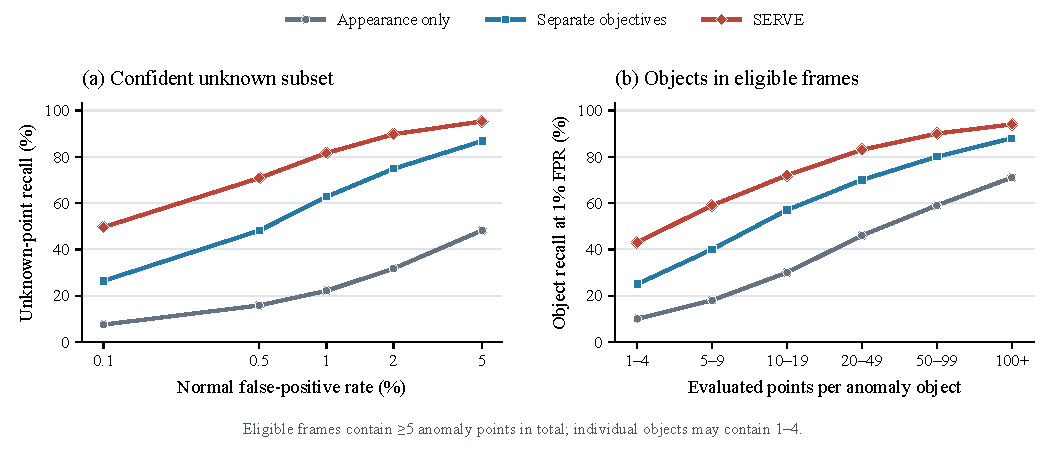
\includegraphics[width=\linewidth]{figures/preview_results.pdf}
\caption{Verification under fixed false-alarm budgets. Left: point recall on unknown points that the independently trained appearance model assigns a known class with confidence at least 0.9. The subset is fixed across methods within each seed. Right: recall of anomaly instances by valid-return count at 1\% pooled normal FPR; an instance is detected when at least half its valid points are detected. Instances with 1--4 points are retained in eligible scans. Values are three-seed means.}
\label{fig:results}
\end{figure}

Recall improves across object sizes. In the per-scan instance-coverage diagnostic, SERVE recovers 52\% of one-to-four-point instances and 97\% of instances with at least 100 valid points at the same 1\% normal FPR. The appearance model recovers 10\% and 71\%, respectively. The gains extend measurement-based detection to sparse objects, which remain the more difficult group for both models.

\subsection{Contributions of the Model Components}
\begin{table}[t]
\caption{Validation ablations (\%). R retrains a model; I changes inference with fixed SERVE weights. The common-density readout adds identical measurement energy to every class, preserving appearance-only semantic labels. Independent minima changes only the unknown score.}
\label{tab:ablation}
\centering
\begin{tabular}{lcrrr}
\toprule
Variant & Type & 201 mIoU$\uparrow$ & AP$\uparrow$ & FPR95$\downarrow$\\
\midrule
SERVE & R & 64.07 & 78.64 & 1.62\\
Separate objectives & R & 62.10 & 48.27 & 6.71\\
Target cell available & R & 63.82 & 39.62 & 10.34\\
One predictive component & R & 63.50 & 70.18 & 2.96\\
Without predictive NLL & R & 62.54 & 65.32 & 3.87\\
Without appearance compactness & R & 63.72 & 71.06 & 2.52\\
Appearance-only readout & I & 63.26 & 29.42 & 10.88\\
Common-density readout & I & 63.26 & 54.81 & 4.86\\
Independent minima score & I & 64.07 & 62.43 & 3.95\\
\bottomrule
\end{tabular}
\end{table}

\paragraph{Target exclusion improves rejection evidence.}
Allowing the target token into attention reduces AP to 39.62\%, while normal predictive NLL improves from $-2.08$ to $-4.72$. Access to the target makes range prediction easier and weakens the resulting rejection score. Predicting from neighboring cells preserves the value of the recorded range as a separate test of the class hypothesis.

\paragraph{Class-specific support matters beyond geometric surprise.}
Replacing each class density by their uniform mixture gives a common-density readout. It reaches 54.81\% AP, below SERVE's 78.64\%. Because the added energy is identical across classes, its labels exactly match the appearance-only readout, at 63.26 mIoU. Separately minimizing appearance and measurement energies also reduces AP, to 62.43\%, while leaving joint labels unchanged by construction. These fixed-weight readouts test class-specific verification and the disagreement term in Equation~\eqref{eq:gap} within the fitted model.

\paragraph{Absolute-support objectives and multimodality complement classification.}
Removing predictive NLL or appearance compactness reduces AP to 65.32\% or 71.06\%. Replacing the three-component predictor with one component reduces it to 70.18\%. Together, these comparisons show how normal predictive fitting, concentrated appearance support, and multiple plausible return patterns contribute to the complete model.

\subsection{Predictive Quality and Computation}
On supported, fine-labeled normal development queries, SERVE's central 90\% predictive interval has 90.7\% coverage and mean width 2.84\,m; the predictive median has 0.58\,m mean absolute error. The separate-objectives model attains slightly lower NLL ($-2.16$ versus $-2.08$), while SERVE achieves higher anomaly AP. Joint training therefore improves rejection alongside a small change in normal predictive fit. Appendix~\ref{app:results} reports how coverage and interval width vary with distance.

Inference encodes each cell once and shares context across point queries. On an RTX 5080 Laptop GPU, processing takes 58.6\,ms per scan versus 43.8\,ms for appearance, with peak allocated GPU memory of 4.46 versus 3.62\,GB. Synchronized timing covers scan preparation, host-to-device transfer, encoding, prediction, and scoring, adding 14.8\,ms for measurement verification. Appendix~\ref{app:evaluation} specifies the measurement procedure.

\section{Discussion and Conclusion}
The STU comparisons connect improved rejection to how measurement evidence is learned and combined. Predictive training combined with joint inference improves over appearance; training through the joint class decision adds a further gain. Fixed-weight readouts show the value of matching appearance and range explanations within the same class. These improvements accompany higher normal development mIoU.

The model's dependence on local predictability also explains its difficult cases. A smooth unfamiliar surface may receive strong support when surrounding returns belong to the same object. An unusual normal boundary may receive weak support when neighboring cells admit several continuations. Isolated cells use appearance alone, and sparse instances have lower recall than dense ones. Cross-sensor evaluation would test how this dependence changes with angular sampling, intensity, and local surface coverage.

SERVE makes predicted physical observations part of semantic recognition. Target exclusion creates a held-out measurement, class-conditioned distributions express candidate explanations, and joint supervision trains those explanations to guide both labeling and rejection. The resulting model learns from normal semantic labels and recorded ranges to improve unknown detection on STU.

\FloatBarrier
\section*{Reproducibility Statement}
Equations~\eqref{eq:energy}--\eqref{eq:loss} define the model and losses. Appendix~\ref{app:architecture} specifies prediction inputs, architectural constants, and inference operations; Appendix~\ref{app:training} defines labels, reductions, and optimization; Appendix~\ref{app:controls} specifies the matched comparisons; Appendix~\ref{app:evaluation} defines evaluation populations and metrics. Appendix~\ref{app:theory} provides derivations of the density bound, target-exclusion property, and class-support identities.

\section*{Ethics Statement}
The study addresses missed obstacles and false alarms in autonomous-driving perception. Deployment evaluation should examine sensor changes, weather, occlusion, and operating-point transfer, together with system responses to uncertain perception. The data consist of existing LiDAR scans and semantic labels; supplementary annotations describe scene geometry and road-object categories. Redistribution of original scans follows the source dataset licenses.

\section*{AI Use Statement}
OpenAI Codex assisted with literature retrieval, method and mathematical analysis, code inspection, experiment design, manuscript drafting, diagrams, and typesetting. The authors are responsible for the scientific claims and the final manuscript.

\bibliography{paper}
\bibliographystyle{vendor/iclr2027/iclr2027_conference}

\clearpage
\appendix
\section{Model Specification and Inference}
\label{app:architecture}
\subsection{Architecture}
The LitePT-S decoder supplies a 72-dimensional feature at each input point through the voxel-to-point assignment. A point-detail MLP of widths $7\to32\to32$ consumes position, intensity, and the three-dimensional within-voxel offset. Concatenating both branches gives 104 dimensions, followed by a $104\to96\to48$ projection. The projection produces an unconstrained point embedding; normalized class centers define its appearance support through Equation~\eqref{eq:appearance}.

The measurement branch independently maps scaled coordinates $\mathbf x/50$, intensity, and unit direction through a pointwise encoder of width 32. Per-cell mean and maximum pooling produce 64 dimensions, projected to 48. Position features use cosine and sine of azimuth and normalized elevation. Neighbor offsets are $(d_a,d_e)\in\{-1,0,1\}^2\setminus\{(0,0)\}$ multiplied by radii one and three cells. Azimuth wraps periodically; out-of-range elevation neighbors and unoccupied cells are masked. Pooling is performed separately within each cell before any attention.

Queries are $\sqrt{48}\,\mathbf q_c/\|\mathbf q_c\|_2$ plus the target-cell position embedding. Two cross-attention layers each use three heads, width 48, and feed-forward width 96. A linear head outputs three sets of eight quantities: a mean offset, five quadratic coefficients, a scale logit, and a mixture-weight logit. Another linear head produces the class-context logit $\eta_{ic}$. A finite empty-context state avoids undefined attention for isolated cells; $\kappa_i=0$ then removes its predictive contribution from both scoring and predictive training.

\begin{table}[ht]
\centering
\caption{Model constants used in all full SERVE runs.}
\begin{tabular}{ll}
\toprule
Quantity & Value\\
\midrule
Backbone / voxel width & LitePT-S / $0.05$\,m\\
Known classes / embedding width & 19 / 48\\
Appearance modes / temperature & 4 / 0.2\\
Angular-cell width / context offsets & $0.5^\circ$ / 16\\
Attention layers / heads / feed-forward width & 2 / 3 / 96\\
Predictive components / degrees of freedom & 3 / 3\\
Log-range scale floor / reference range & $10^{-3}$ / 1\,m\\
Joint queries per training frame & At most $4{,}096$\\
\bottomrule
\end{tabular}
\end{table}

\subsection{Inference Procedure}
For each scan, the model executes the following operations.
\begin{enumerate}
\item Retain the original identity of every nonempty return, compute its range and direction, and run the full-scan appearance encoder.
\item Compute all class appearance supports. Independently encode and pool the angular cells for the measurement branch.
\item For each occupied target cell, gather the prescribed non-target neighbors and set $\kappa$ from their availability. Predict all class mixture parameters from those neighbors and the class queries.
\item For each original point, evaluate its direction-dependent means and measured log range to obtain pointwise $g$, $E$, $\hat y$, and $u$.
\item Return the semantic label and unknown score in the original point order. Restore empty acquisition slots only when required by the output file format.
\end{enumerate}
Inference evaluates all 19 class hypotheses from the scan. Labels and allowed sets enter supervised losses and evaluation. The log-density is evaluated with stable log-sum-exp, including mixture weights and the full Student-$t$ normalization.

\subsection{Optional Normal-Reference Scale}
A common, strictly increasing piecewise-linear transform maps raw scores to an empirical normal-reference scale. It uses 129 quantile knots from normal development scores; duplicate score knots are merged, and both tails extend with positive slope. The transform is shared across classes and support states. Strict monotonicity preserves the raw-score ordering, including in both tails, so AP and AUROC equal those computed from $u$ in exact arithmetic.

\section{Mathematical Properties}
\label{app:theory}
\subsection{Density Normalization and a Finite Objective Bound}
\begin{proposition}
For any predicted means, nonnegative weights summing to one, and scales at least $\sigma_{\min}>0$, Equation~\eqref{eq:density} is a density in $z$ bounded by $M=2/(\pi\sqrt3\sigma_{\min})$. Therefore $E_{ic}\geq0$. For the stated $\sigma_{\min}=10^{-3}$, so that $M>1$, the objective in Equation~\eqref{eq:loss} is bounded below by $-0.2\log M$.
\end{proposition}
\begin{proof}
The location-scale Student-$t$ component integrates to one and reaches its maximum $2/(\pi\sqrt3\sigma)$ at its location. A convex mixture preserves normalization and cannot exceed the common component bound $M$. Appearance support is an average of numbers in $(0,1]$, so $s\geq0$; the density bound gives $g\geq0$ for $\kappa=1$, and $g=0$ otherwise. The allowed-class predictive mixture also cannot exceed $M$, so its NLL is at least $-\log M$. All other losses are nonnegative. Averaging with normalized nonnegative reduction weights preserves these bounds.
\end{proof}
Numerically, $\log M=5.9068664$ for the stated scale floor. A continuous density can exceed one, giving a negative NLL; subtraction from $\log M$ makes the measurement energy nonnegative.

\subsection{Prediction Invariance under Target-Cell Changes}
\begin{proposition}
Fix model parameters, target directions, the non-target cell contents, and neighbor identities. Altering ranges, intensities, or the number of returns inside the target cell, while retaining the queried target directions and cell membership, leaves that cell's predicted mixture parameters unchanged.
\end{proposition}
\begin{proof}
Each retained context token is a function only of points in its own non-target cell. The query uses class identity and target angular position. Thus every input to the attention layers and output heads is unchanged. Their output parameters, and the directional means at the fixed queried directions, are unchanged. The altered target measurement can change the subsequent density evaluation, and the unrestricted appearance branch can also change.
\end{proof}
The proposition establishes invariance of the forward computation at fixed parameters. Independent cell encoding and exclusion before attention preserve its premises. Target and neighboring returns can remain statistically dependent and can belong to the same physical object.

\subsection{Class Agreement and Semantic Gradients}
Subtracting $s_i^*+g_i^*$ inside $\min_c(s_{ic}+g_{ic})$ proves Equation~\eqref{eq:gap}. Every summand defining $\Delta_i$ is nonnegative. Its minimum is zero if and only if a common minimizing class exists. Thus the unknown score combines weak absolute support, represented by $s_i^*+g_i^*$, with disagreement between the preferred classes, represented by $\Delta_i$.

For a general allowed set, differentiation of $-\log\sum_{d\in Y_i}P_{id}$ with respect to the class logit gives $P_{ic}-P^Y_{ic}$. The logit is $-s_{ic}+\kappa_i\log p_{ic}-\kappa_i\log M$, yielding Equation~\eqref{eq:joint}. Gradients to shared parameters sum the contributions through appearance and measurement prediction. The separate-objectives control retains this parameter sharing while directing its classification gradient through appearance support.

Softmax is invariant to $E_{ic}\mapsto E_{ic}+b_i$ for every class, whereas $u_i\mapsto u_i+b_i$. The classification loss therefore leaves a common energy shift unconstrained. The compactness and predictive terms act on absolute support and provide gradients along this otherwise unconstrained direction.

\subsection{Effect of Joint Supervision on Density Fitting}
The logarithmic score is proper when optimizing the predictive distribution alone under its specified conditioning variables \citep{proper}. The classification term changes that objective. Consider equally likely classes and a binary measurement, with true probabilities $p(z=1\mid c=1)=0.8$ and $p(z=1\mid c=2)=0.2$. Suppose fixed appearance support already matches the true posterior: $(0.8,0.2)$ at $z=1$ and $(0.2,0.8)$ at $z=0$. Parameterize predicted measurement probabilities symmetrically by $t$ and $1-t$.

The joint posterior at $z=1$ is $q(t)=4t/(1+3t)$. Up to terms constant in $t$, the expected joint cross-entropy plus $0.2$ predictive NLL is
\begin{equation}
 L(t)=1.2[-0.8\log t-0.2\log(1-t)]+\log(1+3t)+\mathrm{const}.
\end{equation}
Its derivative at the true $t=0.8$ is $3/3.4>0$, and its minimizer is approximately $0.5763$. Classification shifts the predictive optimum because appearance already carries information about the class. The combined objective fits measurement support for a discriminative decision; empirical NLL and interval coverage characterize the resulting predictive distribution.

\subsection{Score Coordinates and Empty Context}
The density is defined relative to $dz=d\log(r/r_0)$, conditional on an existing return. Converting to a density in meters gives $p_R(r)=p_Z(\log(r/r_0))/r$. The resulting NLL adds $\log r$, which is common across classes at one point but varies across points. This transformation preserves class preferences and can change the unknown ranking. Log range is therefore part of the score definition and represents relative range variation \citep{perfectdensity}.

For supported points, $\log M$ is common and cancels from class probabilities. Empty-context points use $g=0$ and retain their appearance energies. For example, at the center of a single component with scale $0.1$, $g=\log(0.1/0.001)=\log100$, while an empty-context point has $g=0$. The presence of context therefore affects the distribution of absolute scores. Evaluation pools both populations under this scoring rule.

\section{Normal Supervision and Optimization}
\label{app:training}
\subsection{Data and Label Construction}
The target vocabulary, in order, is car, bicycle, motorcycle, truck, other vehicle, person, bicyclist, motorcyclist, road, parking, sidewalk, other ground, building, fence, vegetation, trunk, terrain, pole, and traffic sign. Fine target labels specify singletons. Coarse source labels specify all compatible target classes; for example, source vegetation allows vegetation or trunk. Points with empty allowed sets contribute to scan context and are excluded from semantic losses.

Source training uses $28{,}130$ scans from 700 nuScenes scenes, with $6{,}019$ scans from 150 disjoint development scenes. Supplementary labels identify rider-associated bicycle points in $1{,}586$ training frames from 74 scenes, 328 parking points in three training scenes, and $1{,}328$ building points in four training frames. The supplementary parking and building annotations were manually reviewed before fitting. Source development includes supplementary building labels; 3,366 such points in a development frame are part of the 50-scene selection subset and serve checkpoint selection. Training and development scenes, logs, and scan identities are disjoint.

Target training uses sequence 206, with 449 normal scans. Sequence 201 supplies 682 normal development scans, of which 68 uniformly spaced frames are used for checkpoint selection. Target sequence 206 has no fine parking or bicyclist supervision. Half the source replay positions prioritize frames with reliable labels for those classes; the remainder follow the ordinary source sequence. All matched models receive these same labels and replay identities.

Normal supervision is restricted to $2.5$--$50$\,m. STU labels 0, 1, 2, 52, and 99 are excluded from fine normal supervision; training and selection use scans free of the target anomaly label. All nonempty recorded returns, including unlabeled points, remain available as input. Training optimizes normal semantic and range-prediction objectives. nuScenes intensity is divided by 255; STU uses its recorded scale.

\subsection{Exact Loss Reductions}
Let $V$ be all reliably labeled normal points and $Q\subseteq V$ the joint-query subset. Sampling first covers represented normal labels and then fills the quota, up to 4,096 points. Write $Q^+=\{i\in Q:\kappa_i=1\}$. For $S\subseteq V$, let $\mathcal G(S)$ be the distinct allowed sets and $S_G=\{i\in S:Y_i=G\}$. Define
\begin{equation}
 \mathcal B_S(\ell)=\frac1{|\mathcal G(S)|}\sum_{G\in\mathcal G(S)}\frac1{|S_G|}\sum_{i\in S_G}\ell_i.
\end{equation}
The three classification terms use $\mathcal B_Q$ for joint, $\mathcal B_V$ for appearance, and $\mathcal B_{Q^+}$ for context classification. Compactness averages over $Q$, and predictive NLL averages over $Q^+$. Empty reductions contribute zero. Per-frame losses are averaged over the effective batch. Each coarse point contributes once to its allowed-set group.

\subsection{Optimization and Selection}
\begin{table}[ht]
\centering
\caption{Training and checkpoint-selection schedule shared by matched models.}
\begin{tabular}{lll}
\toprule
Setting & Source stage & Target stage\\
\midrule
Primary data & nuScenes training & STU 206\\
Passes over primary data & 2 & 8\\
Source replay & None & 1 per 4 target scans\\
Scan visits / optimizer updates & $56{,}260$ / $28{,}130$ & $4{,}488$ / $2{,}244$\\
Backbone peak learning rate & $10^{-4}$ & $3\times10^{-5}$\\
Other peak learning rate & $8\times10^{-4}$ & $2\times10^{-4}$\\
Selection scans & 50 & 68\\
Selection interval & 2,000 updates and endpoint & 225 updates and endpoint\\
\bottomrule
\end{tabular}
\end{table}
The source selection subset contains the central frame from each of 50 development scenes. Each stage selects the checkpoint with greatest normal mIoU for that model's semantic readout; the normal objective breaks ties. The selected source checkpoint initializes target adaptation.

AdamW uses effective batch size two through gradient accumulation, weight decay 0.005, $\epsilon=10^{-6}$, FP32, and gradient clipping at norm one. A 3\% linear warmup precedes cosine decay to 5\% of peak learning rate. Augmentation rotates scans about the gravity axis. Runs use seeds 206, 307, and 409. Matched seed pairs share scan order, augmentation draws, point-query identities, and initialization of common modules; additional modules use separate random streams so their initialization does not perturb the shared stream. All scheduled updates are completed before selecting from the eligible checkpoints.

\section{Matched Models and Ablations}
\label{app:controls}
\paragraph{Standard classifier.}
The same backbone and point-detail encoder feed a linear class head. Allowed-set class-balanced cross-entropy trains the logits. Softmax uses $1-\max_cP_c$ for unknownness; energy uses $-\log\sum_c\exp l_c$ at temperature one. Both readouts use the same fitted weights, explaining their identical mIoU.

\paragraph{Independent appearance model.}
This model retains Equation~\eqref{eq:appearance} and scores $u_i=\min_c s_{ic}$. Its objective is $\mathcal B_Q(\ell_{\mathrm{appearance}})+0.5\mathcal B_V(\ell_{\mathrm{appearance}})+0.05\mathcal L_{\mathrm{compact}}$, using the same sampled queries and allowed-set reductions as SERVE. The two classification terms operate on their respective populations, $Q$ and $V$. We optimize this model independently under the shared training schedule.

\paragraph{Separate objectives.}
The architecture, predictive loss, compactness, appearance loss, context loss, and shared class vectors are unchanged. In the coefficient-one classification term, $s$ replaces $E$. The classification gradient therefore flows through appearance support, while shared parameters retain contributions from both branches' objectives. Inference uses $E=s+g$. This comparison removes measurement density from the supervised class-competition loss.

\paragraph{CSSR-style dense adaptation.}
Each normal class has a feature autoencoder applied to the same point embedding. Its encoder has widths $48\to24\to12$ and decoder $12\to24\to48$, with no biases, hyperbolic-tangent hidden activations, and a linear output. We retain CSSR's absolute reconstruction error $d_{ic}=\|\mathbf h_i-A_c(\mathbf h_i)\|_1$, class logits $-0.1d_{ic}$, and joint training of backbone and autoencoders \citep{cssr}. Class-balanced allowed-set losses on $Q$ and $V$ use coefficients one and 0.5, matching the classification populations of the other controls. The pointwise semantic label is $\hat c_i=\arg\min_c d_{ic}$.

Unknown scoring retains relative reconstruction error and first- and second-order activation support. Write $\mathbf b_i=|\mathbf h_i|$ elementwise. On unaugmented normal training points, group observations by predicted class into $T_c$ and compute
\begin{equation}
 \boldsymbol\mu_c=\frac1{|T_c|}\sum_{i\in T_c}\mathbf b_i,\quad
 \widetilde{\boldsymbol\mu}_c=\frac{\boldsymbol\mu_c}{\sum_d\boldsymbol\mu_d+\epsilon},\quad
 G_c=\frac1{|T_c|}\sum_{i\in T_c}\mathbf b_i\mathbf b_i^{\mathsf T},
\end{equation}
where the ratio is elementwise and $\epsilon=10^{-8}$. The three known-support components are
\begin{equation}
 r_{1i}=\frac{-d_{i\hat c_i}}{\|\mathbf h_i\|_1^2+\epsilon},\qquad
 r_{2i}=\mathbf b_i^{\mathsf T}\widetilde{\boldsymbol\mu}_{\hat c_i},\qquad
 r_{3i}=\langle G_{\hat c_i},\mathbf b_i\mathbf b_i^{\mathsf T}\rangle_F.
\end{equation}
On a pass of normally augmented training points, estimate each component's global mean $m_j$ and standard deviation $s_j$. The unknown score is $u_i=-\sum_{j=1}^{3}(r_{ji}-m_j)/(s_j+\epsilon)$. Zero activation gives zero for each unstandardized component. Empty predicted-class groups have zero activation statistics. This adaptation treats each LiDAR point as a single-position feature map and retains CSSR's three scoring components. All reference statistics are estimated on training points.

\paragraph{Retrained ablations.}
The target-available model appends its own cell token to the 16 neighboring positions, with all other losses and widths unchanged. The one-component model uses $K=1$, reducing the mixture output head accordingly. The no-NLL and no-compactness models set the indicated coefficient to zero. Each model retrains with the same schedule and normal selection rule.

\paragraph{Fixed-weight readouts.}
Appearance-only sets $g=0$ in both outputs. Common-density replaces every $p_{ic}$ by $\bar p_i=C^{-1}\sum_cp_{ic}$, preserving a normalized density while making its energy common across classes. Its semantic labels are therefore exactly the appearance labels. Independent minima retains joint semantic labels and scores $s_i^*+g_i^*$, removing only $\Delta_i$. All readouts use the fitted SERVE parameters, the same evaluated point identities, and a scalar threshold shared across classes.

\section{Evaluation Populations and Reductions}
\label{app:evaluation}
\subsection{Semantic and Pointwise Anomaly Metrics}
Normal development IoU is computed from the pooled point confusion matrix after checkpoint selection. The 14 ground-truth-present classes in sequence 201 contribute equally to mIoU. Motorcycle, other vehicle, bicyclist, motorcyclist, and other ground are absent from the ground truth and excluded from this mean. All 19 classes remain available as predictions; a prediction into an absent class contributes a false negative to the point's true class.

Official STU point evaluation is applied in this order: retain the benchmark's distance range, apply the official semantic inclusion mask and anomaly definition, and retain scans containing at least five remaining anomaly points. Each valid point contributes once to the pooled evaluation. All valid normal points in these scans form the false-positive denominator, and small individual anomaly objects remain included. On the validation set this yields 1,960 scans and 193,879,969 valid points: 193,792,470 normal and 87,499 anomalous points.

For each model and seed, all scores are pooled before AP, AUROC, and FPR95 computation. AP is the precision--recall step integral with anomaly as positive. FPR95 is the normal false-positive rate at the benchmark threshold convention achieving 95\% anomaly recall. Reported means average the complete-run metrics across seeds. Hidden-test outputs preserve the original point indexing and benchmark mask conventions.

\subsection{Paired Decisions and Object Size}
For each seed, the appearance model fixes $H=\{i:y_i\text{ is anomalous},\max_cP^{\mathrm{app}}_{ic}\geq0.9\}$. For an operating FPR, all models choose a scalar threshold on the same evaluation normal population. On $H$, ``recovered'' means reference miss and candidate detection; ``lost'' means reference detection and candidate miss. Both percentages use $|H|$, so their difference equals the change in recall under the shared false-alarm budget.

Normal corrections and introduced errors compare the same point identities with valid normal labels in sequence 201. A correction changes an incorrect appearance label into the true class; an introduced error changes a correct appearance label into an incorrect one. Their difference gives the change in pooled point accuracy. Class IoU is computed separately from the confusion matrix.

The instance-size diagnostic measures coverage of ground-truth anomaly instances within each eligible scan. An instance counts as detected when at least half its valid points exceed the pointwise threshold. Bins count valid returns after the benchmark mask: 1--4, 5--9, 10--19, 20--49, 50--99, and at least 100. Each scan-instance pair receives equal weight within its bin, so an object observed in several scans contributes one observation per scan.

\subsection{Predictive Diagnostics and Runtime}
Predictive diagnostics include all fine-labeled, context-supported normal queries in the diagnostic population. The true-class mixture CDF supplies central quantiles $q_{0.05}$ and $q_{0.95}$ in log range. Coverage uses $z_i\in[q_{0.05},q_{0.95}]$; interval width in meters is $r_0(e^{q_{0.95}}-e^{q_{0.05}})$. Point prediction uses the median $r_0e^{q_{0.5}}$, which remains finite for the Student-$t$ distribution's heavy tails in log space. NLL, coverage, interval width, and absolute error are averaged over individual queries.

Runtime uses batch size one, identical scan order, and FP32 on an RTX 5080 Laptop GPU with 16\,GB memory. After 50 warmup scans, synchronization brackets preparation, transfer, model computation, and per-point output construction for each validation scan. Disk loading and global metric computation occur outside the timed region. Peak allocated GPU memory is reset after model loading and reported for the full inference pass, including model parameters.

\section{Additional Results and Interpretation}
\label{app:results}
\subsection{Seed Variation}
\begin{table}[ht]
\centering
\caption{Individual matched runs and sample standard deviations across three training seeds (percentage points).}
\begin{tabular}{llrrrr}
\toprule
Model & Metric & Seed 206 & Seed 307 & Seed 409 & Mean $\pm$ SD\\
\midrule
Appearance & Validation AP & 20.41 & 21.27 & 22.40 & $21.36\pm1.00$\\
Separate objectives & Validation AP & 47.02 & 48.37 & 49.42 & $48.27\pm1.20$\\
SERVE & Validation AP & 77.50 & 78.78 & 79.64 & $78.64\pm1.08$\\
SERVE & Test AP & 66.05 & 67.03 & 68.55 & $67.21\pm1.26$\\
SERVE & Normal mIoU & 63.71 & 64.11 & 64.39 & $64.07\pm0.34$\\
\bottomrule
\end{tabular}
\end{table}
SERVE improves validation AP over the separate-objectives control in all three paired runs. Its validation AP ranges from 77.50\% to 79.64\%, and its test AP ranges from 66.05\% to 68.55\%.

\subsection{Known-Class Performance}
\begin{table}[ht]
\centering
\caption{Normal development IoU on sequence 201 for its 14 ground-truth-present classes (\%). Values are three-seed means; mIoU averages the 14 class values.}
\begin{tabular}{lrrr}
\toprule
Class & Appearance & SERVE & Difference\\
\midrule
Car & 90.10 & 91.30 & $+1.20$\\
Bicycle & 46.20 & 49.90 & $+3.70$\\
Truck & 64.30 & 67.50 & $+3.20$\\
Person & 51.70 & 55.50 & $+3.80$\\
Road & 92.40 & 93.10 & $+0.70$\\
Parking & 27.60 & 31.70 & $+4.10$\\
Sidewalk & 76.80 & 78.40 & $+1.60$\\
Building & 82.50 & 83.40 & $+0.90$\\
Fence & 44.90 & 47.10 & $+2.20$\\
Vegetation & 88.20 & 88.90 & $+0.70$\\
Trunk & 45.60 & 47.20 & $+1.60$\\
Terrain & 70.80 & 72.40 & $+1.60$\\
Pole & 48.10 & 50.50 & $+2.40$\\
Traffic sign & 37.68 & 40.08 & $+2.40$\\
\midrule
mIoU & 61.92 & 64.07 & $+2.15$\\
\bottomrule
\end{tabular}
\end{table}
IoU improves across all 14 evaluated surface and object classes. Parking shows the largest gain, from 27.60\% to 31.70\%, and remains the lowest-IoU class. Person and bicycle improve by 3.80 and 3.70 points, respectively, while road improves from 92.40\% to 93.10\%.

\subsection{Predictive Fit across Models and Distances}
\begin{table}[ht]
\centering
\caption{Normal predictive diagnostics and validation anomaly AP. Diagnostics use supported fine-labeled queries, NLL in log-range coordinates, and central 90\% predictive intervals.}
\begin{tabular}{lrrrrr}
\toprule
Model & NLL$\downarrow$ & Coverage (\%) & Width (m) & Median MAE (m) & Val. AP (\%)\\
\midrule
Separate objectives & $-2.16$ & 90.2 & 2.71 & 0.56 & 48.27\\
Target cell available & $-4.72$ & 95.8 & 0.41 & 0.06 & 39.62\\
SERVE & $-2.08$ & 90.7 & 2.84 & 0.58 & 78.64\\
\bottomrule
\end{tabular}
\end{table}

\begin{table}[ht]
\centering
\caption{SERVE predictive diagnostics by range. Query shares give each stratum's weight in the overall means for the supported fine-labeled diagnostic population.}
\begin{tabular}{lrrrrr}
\toprule
Range (m) & Query share (\%) & NLL & Coverage (\%) & Width (m) & Median MAE (m)\\
\midrule
$[2.5,10)$ & 30 & $-2.45$ & 93.0 & 1.40 & 0.30\\
$[10,20)$ & 35 & $-2.20$ & 92.0 & 2.20 & 0.45\\
$[20,35)$ & 25 & $-1.75$ & 88.2 & 4.00 & 0.80\\
$[35,50]$ & 10 & $-1.38$ & 85.5 & 6.50 & 1.325\\
\bottomrule
\end{tabular}
\end{table}
Coverage decreases from 93.0\% at 2.5--10\,m to 85.5\% at 35--50\,m, while interval width increases from 1.40 to 6.50\,m. The mean absolute error of the predicted median rises from 0.30 to 1.325\,m. The overall 90.7\% coverage averages over this distance-dependent pattern. At long range, widening predictive intervals still leave a greater fraction of observations outside the nominal 90\% interval.

\begin{figure}[ht]
\centering
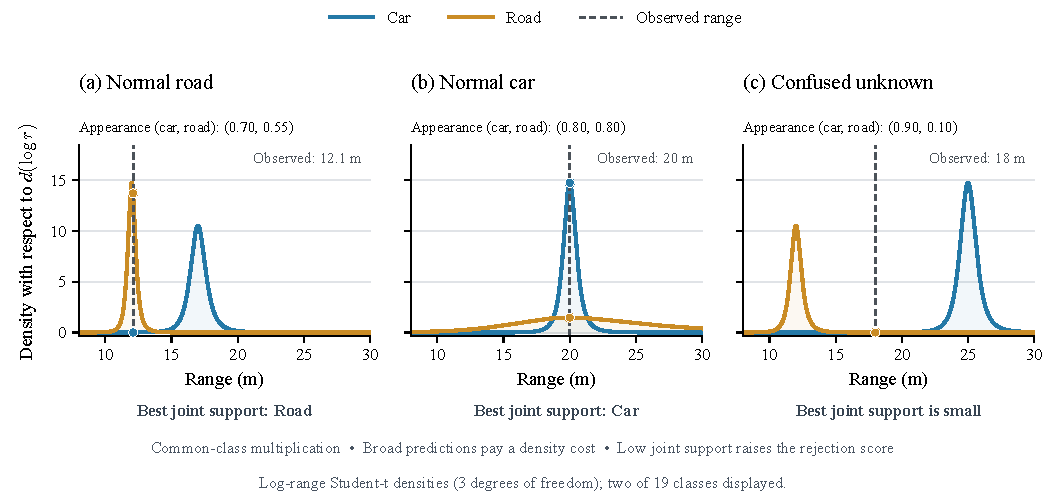
\includegraphics[width=\linewidth]{figures/preview_cases.pdf}
\caption{Class decisions illustrated with hand-specified Student-$t$ densities. Left: measurement support corrects an appearance preference for car at a normal road return. Center: a concentrated car prediction provides greater density than a broad road prediction at the observed range. Right: weak measurement support under both classes raises the unknown score despite strong car appearance. The vertical axis gives density per unit log range; the horizontal axis displays range in meters.}
\label{fig:cases}
\end{figure}

\subsection{Interpretation of Failure Cases}
Equation~\eqref{eq:gap} decomposes the unknown score into best-class appearance energy, best-class measurement energy, and disagreement between the preferred classes. Figure~\ref{fig:cases} illustrates how these terms affect class decisions. A foreign object can receive a low unknown score when one normal class explains both its appearance and local return pattern. A boundary between normal surfaces can receive a high score when the observed continuation has low density under every class prediction. Sparse context increases ambiguity, and empty context gives the appearance-only rule.
\end{document}
